\section{Critique of the Information Ecosystem}

Information ecosystems and information ecologies share much more than the root of the word ecology. Information ecology outlines programs for research that borrows ecological concepts and applies them in information science.  The metaphor of the information ecosystem imparts notions of evolution, connectivity, diversity, complexity, dynamic equilibriums, keystone species, and even predator prey relationships. Thus far we have explored how these concepts have emerged both in ecology as a discipline and in several "ecological" approaches to research in other fields. As shown, there is much overlap between ecology and information science as the two disciplines came into being in the postwar academy. Ecology borrowed ideas about diversity, cybernetics, and systems thinking from information science and information science is now seeking ecological approaches to digital resource management. This cross-fertilization has been very productive in terms of generating new knowledge about these phenomena, both natural (ecology) and social (information science). 

The reminders that technical solutions are embedded in social contexts found in the work of Nardi, Davenport, and even Lucas  are timely and important. The broad focus on the interdisciplinary management of resources, both natural and digital, deserves more attention. The interplay between information science and ecology around mathematical models of diversity, cybernetic theory, dynamic equilibriums, and chaotic systems with tipping points continues to produce novel insights and management methods. Finally the idea that everything is connected and somehow interdependent is powerful indeed.

On the other hand the role that data and information play as a conduit between social phenomena and the natural world tends to get lost somewhere in the information ecosystem metaphor. The information itself becomes the environment and the natural environment fades into invisibility. Instead of speaking to sustainability of socio-natural systems, sustainability is expressly narrow to economic terms. Furthermore the naturalizing of human communities through the metaphor of the information ecosystem in a scholarly context, or the scholarly ecosystem, is problematic. Perhaps even more problematic is that through an information ecology, human built systems for the management of information somehow become naturalized, out of our control, emergent, and perhaps even evolving.

\subsection{Human Communities are not Ecosystems!}

One of the uses of the ecosystem metaphor in research data management and scholarly communication circles is that scholarly communities are like "ecosystems" through which rivers of data flow \citep{choudhury_2010}. This use of the metaphor invokes a very appealing image of librarians tending the flows of data which pass through scholarly ecosystems nestled within the green hills of the academy. It is perhaps also a dangerously comforting image that borderlines on committing the \textit{Naturalistic Fallacy}; because things are found in nature, they are good \citep[see][p. 68 for a similar example in business management]{lucas_2012}. Cognitive scientist Steven Pinker counters this fallacy by noting that possible logical conclusions include statements such as, "if birds and beasts engage in adultery, infanticide, and cannibalism, it must be OK" \citep{pinker_2002}. 

Another analogous use of the metaphor is that the library itself is an ecosystem in which library specialists, library users, and library professionals interact as different species who have both "competing interests" and relations of "mutual benefit". These relationships lead to a co-evolution of the "species" in a rapidly changing research, publishing and technology environment \citep{walter_2008}. At a broader scale some authors suggest that even human economies should be thought of as ecologies (as a set of relations) \citep[][p. 72]{lucas_2012}. Once again this evokes a sort of touch-feely image where mutualism and cooperation inevitably lead to some sort of outcome that benefits all the "species" involved. 

Scholarly communities, be it the research community or the library community, are hierarchical, much like a government agency, with politics and power rippling through their ranks. It is discomforting to think that that, with just a little stretching of these metaphors, the US Department of Defense, or some other government agency, is like an ecosystem through which data flows naturally. The solace to be found with this discomfort comes from the words of Richard Stallman: “It is inadvisable to describe the free software community, or \textit{any human community}, as an “ecosystem,” because that word implies the absence of ethical judgment.”  Stallman continues:
 
\begin{quote}
The term “ecosystem” implicitly suggests an attitude of nonjudgmental observation: don't ask how [sic] what should happen, just study and understand what does happen. In an ecosystem, some organisms consume other organisms. In ecology, we do not ask whether it is right for an owl to eat a mouse or for a mouse to eat a seed, we only observe that they do so. Species' populations grow or shrink according to the conditions; this is neither right nor wrong, merely an ecological phenomenon, even if it goes so far as the extinction of a species.

By contrast, beings that adopt an ethical stance toward their surroundings can decide to preserve things that, without their intervention, might vanish—such as civil society, democracy, human rights, peace, public health, a stable climate, clean air and water, endangered species, traditional arts … and computer users' freedom. \citep{fsf_2014}
\end{quote}

Perhaps these words also apply to information systems—as these systems are indeed social phenomena—and although the ecosystem metaphor may be convenient and perhaps even practical to describe a scholarly community, we should be careful with expressing an implicit lack of morality in the world of information. 

\subsection{Data as a natural phenomena}

An ecosystem or ecology (as a set of relations) is an abstraction of nature and the relationships between living organisms and their surrounding non-living environment. While living organisms, including humans, have a dialectical relationship with ecosystems--organisms influence the ecosystem and the ecosystem influences organisms--an ecosystem is not purposefully made by the organisms for material exchange. On the other hand we know that markets are purposefully built for economic exchange. We can only wonder if nature has such purpose \citep{glacken_1967}. To reduce an ecosystem to human-made, such as an information ecosystem, denies possibilities of spiritualism and non-quantifiable relationships that we have with nature.

In the recent book \textit{Trillions} there is an allusion that the rules of the Internet that were created to manage complexity are analogous to the rules of nature in an ecosystem. While the authors admit that if we are "to play god by creating an ecology ... the first requirement ... is humility", the assumption that we create instead of manage ecosystems is controversial \citep[][p. 140]{lucas_2012}. Is there the possibility of the emergence of life in the information ecosystem? Does linking emergence to biological and environmental concepts benefit our understanding of novel information systems? With the information ecosystem metaphor de we suggest that we have finally reached the status of a god and created a new form of life? Furthermore, this allusion naturalizes the Internet in the sense that the rules are not open to change by the common user or indeed anyone else. Only the \textit{gods} of the Internet have the privilege to modify these rules. 

Furthermore, if the rules of the internet are natural does that imply that data found on the internet is natural? In a recent UK publication that outlines digital reseach methods, Big Data is defined as "‘naturally occurring’, high-volume digital data which are often available in ‘real-time’ and which are not produced with social scientific research as an objective" \citep{ncrm_2015}. Or as appeared in Forbes magazine: "The real impetus is the potential insights we can derive from this new, vast, and growing \textit{natural} resource." \citep[][emphasis ours]{rotella_2012}. Within these statements it is completely obviated that we collect data from natural and social environments; it is not given to us as a natural phenomena, but something we chose to gather, interpret, and use to make sense of the environment \citep{kitchin_2014}.

Within certain critical academic circles naturalizing a phenomena that is a human creation—somehow perceiving the social phenomena as natural—is considered dangerous. A good example might be an explanation of the conquest of Peru as inevitable and ‘natural’ because of superior European weaponry and the disease trajectory from Europe to South America (to simplify a famous argument). Nowhere in this explanation is it mentioned that the conquistadors were social outcasts with a tendency for violence and disrespect of life; perhaps another factor in the conquest. Does emotional analysis of Twitter data really represent the human condition? Do market analytics of Amazon purchases represent a natural phenomena, especially if you consider the human created commercial aparatus that drives those purchases?  

\subsection{Green[wash]ing the information economy:}

It is hard to argue that anything ecological is bad. While never stated directly as a tactic to greenwash computing, the information ecology in Nardi and O'Day's work is strongly suggestive: if the use of computers is part of an ecology, then critique becomes more difficult, computers become more friendly, and information systems form part of everything good. While they were writing in the 1990s before the Internet and world wide web became one of the dominant information forces in the world, this period also marked the consolidation of the neoliberal Washington consensus in the economic and political realms.

\textit{Trillions} also makes a strong argument that the purpose of the information ecology metaphor (as a set of relations) is to bring humans back into the solution. Like Nardi and O'Day they focus on human-centric design, less visible technologies, and so on \citep{lucas_2012}. Their work is a thinly veiled conservative argument for the 'liberation' of information in the sense that there should be no regulation; the information ecology (as a set of relations) will be self-regulating, based in free-market neoliberalism, and of course will generate huge opportunities for business. It is almost as though they use the word ecology instead of economy because they know with 'economy' the veil will disappear.

As data becomes liberated and flows more freely our ability increases to capture larger quantities of data. Does the quality of catpured data decline? As Niel Postman suggests, "We have transformed information [and data] into a form of garbage" \citep[cited in][p. 50]{stepp_1999}. Does this potential decline in quality information somehow hamper effective decision making or are we able to filter and analyze the data in ways that provide novel insights that improve effective decision making? Or as Barend Mons put it recently, "Data is like oil. We pump it from the earth. We spill it everywhere. We make a mess" \citep{mons_2016}. 

If these observations ring true, how long will it be until negative environmental outcomes of high flow liberated data will become apparent? The "cloud" is literally tons of spinning metal disk that resides in an air-conditioned complex. All of our information technologies draw natural resources from the environment (metal, plastic, energy, and rare earth minerals), and then after several years of use, become a waste stream that returns to the environment. In many parts of the world extraction and recycling are unregulated industries with negative environmental and social impacts.

\subsection{Sustainable resource management}

A common thread in all of the literature reviewed is that of resource management, be the resources digital or natural. From the information ecology literature we see the emphasis on context, particularly political and economic, for the best management of data. This resonates particularly well with the literature from political ecology and its project to contribute to sustainability studies with the allied fields in geography of land use land change and socio-ecological systems. Management prescriptions from this work emphasize adaptive management cycles where assessment leads to planning and doing followed by evaluation and back to assessment \citep{holling_1978,liu_etal_2007}. Attention to system disturbance and potential shifts from dynamic equilibriums to periods of chaotic behaviour is shared between the adaptive management literature and the information ecology programs outlined by Nardi, Davenport and their co-authors. 

An interest in sustainability is also shared and several leading scholars in different fields have made progress in linking natural resource management with the management of digital resources, largely through thinking about forms of property. Elinor Ostrom, who published on the sustainable management of natural resources for over two decades, turned her focus to digital resources and with librarian Charlotte Hess and published on the knowledge commons at the end of her career \citep{hess_2006}. Her work on ownership regimes and sustainable management is a powerful argument for the importance of common property resources in sustainable systems, even in a time where private property tends to be the mainstream prescription. Hers is an argument against the "Tragedy of the Commons" thesis whereby common property regimes beget environmental degradation.

The legal scholar, James Boyle, tackles the same problem from the perspective of intellectual property rights and the management of material in the public domain. His straw man is that "words can be overgrazed" and therefore must be protected by private property, but with careful analysis he shows that this is not true and the public domain is ever more important in a digital age \citep[][footnote 15 on p. 5]{boyle_2003}. His concerns over increasing corporate ownership of scholarly output are also applicable to data; it is likely that data cannot be "overgrazed" and that balanced public/private ownership of data will be a key for sustainable data management. Even the economist Joseph Stiglitz, ex-president of the world bank, sees the need for balanced ownership regimes where over-emphasis on copyright and private ownership can damage knowledge as a global public good \citep{stiglitz_1999}.

\subsection{Disappearing Nature}

There is a confusion of ecology with ecosystems, and both with economies \citep[cf. ][]{lucas_2012,nardi_information_1999}. Similar to ecosystems, economies draw material wealth from nature: stocks and flows of natural resources, minerals, water, energy and so on. But in classical economics it is often forgotten that resource streams and waste flows take place within an ecosystem. Yet from the perspective of ecological economics the economy is entirely dependent on nature and indeed is a human-created subsystem of natural processes (see figure 4).

\begin{figure}[!ht]
  \centering
    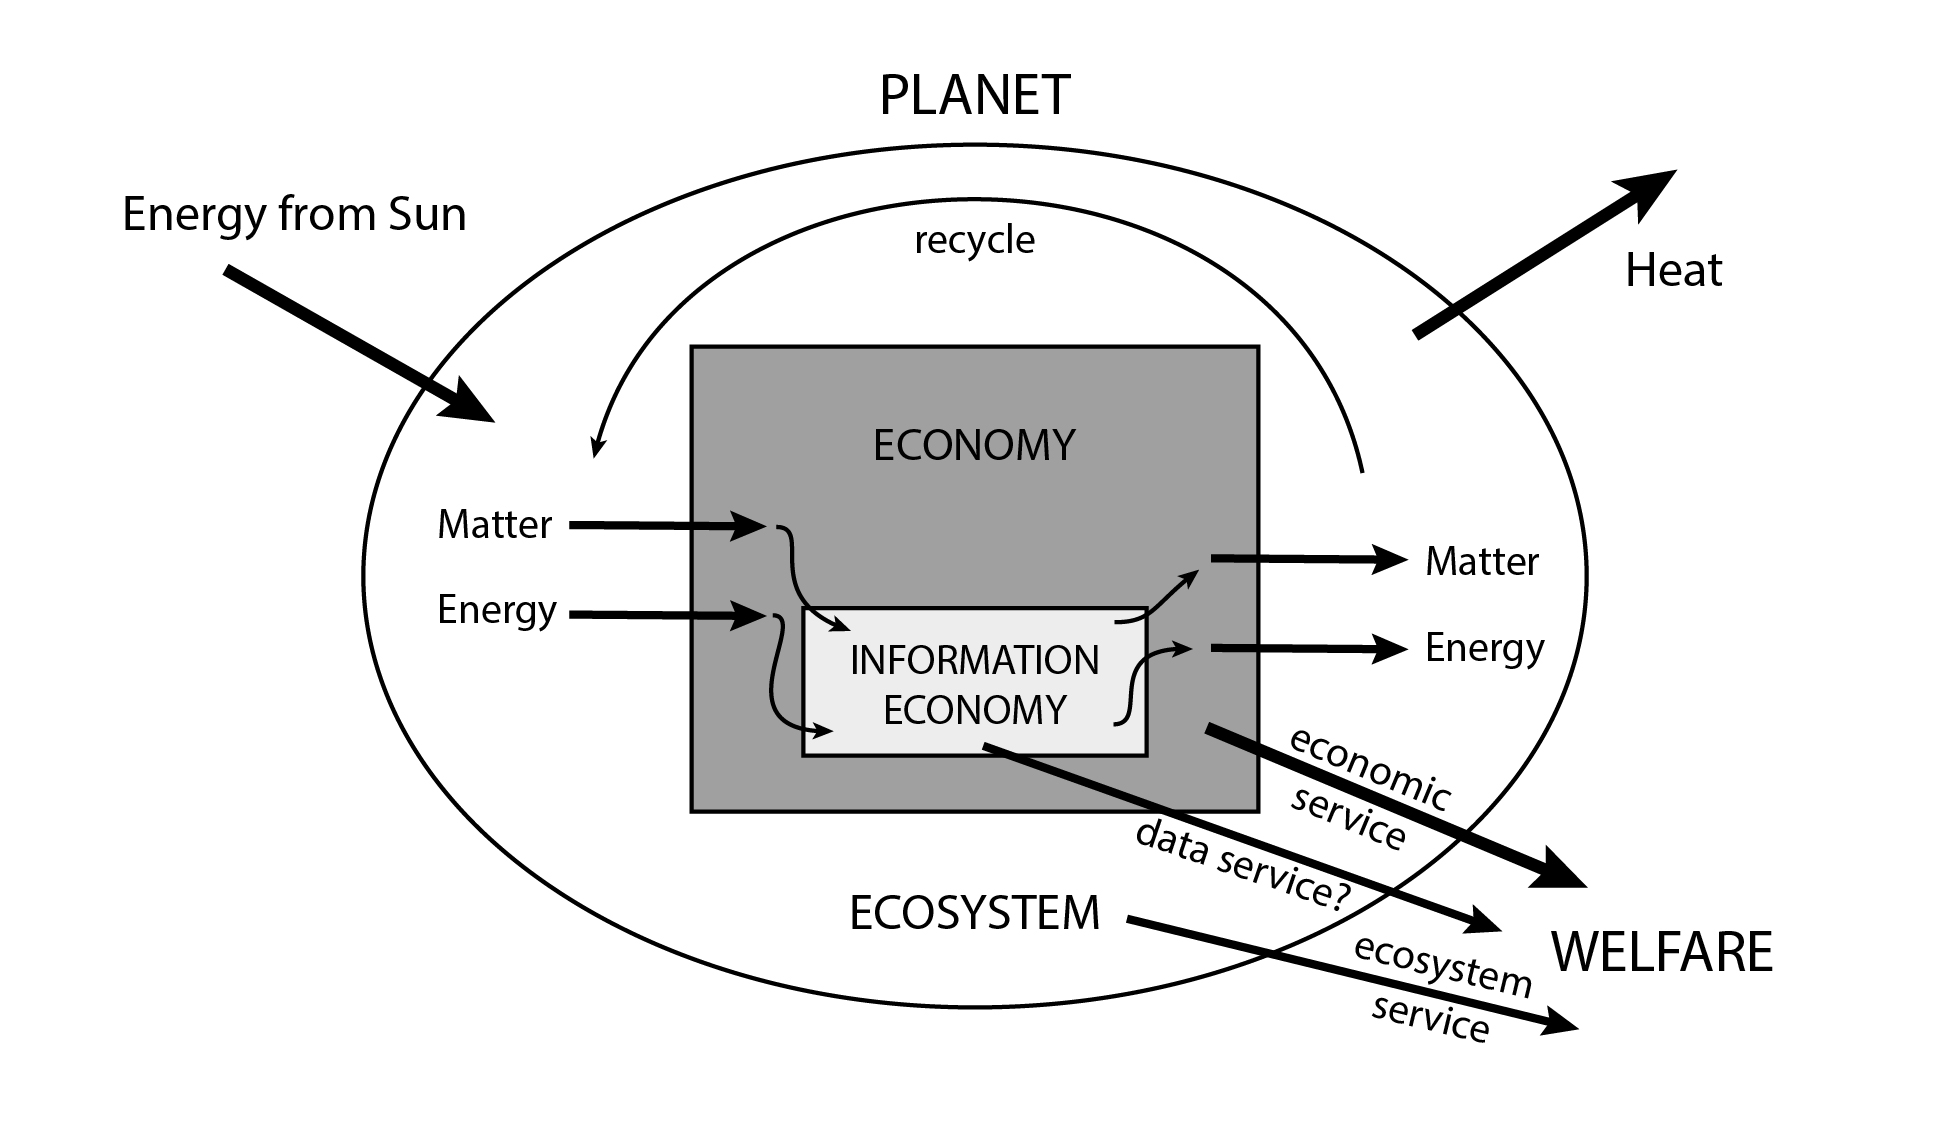
\includegraphics[width=5.5in]{figures/ecologicalecon}
  \caption{The information economy understood as a sector of the global economy which itself is a sub-system of the global ecosystem. Adapted from \citep[][p. 18]{daly_2004}}
\end{figure}

Through the claim that the information system is an ecology (as a set of relations) instead of an economy, natural ecosystems become even less visible. The very real need for natural resources such as energy, metal, petroleum, and space itself to build and maintain information systems fade into the background of the conversation. Our incomplete review of the literature suggests the possiblity that the use of the term "information ecosystem" or "information ecology" (as the relations) further disconnects us from our natural environment.  This disconnection may indeed be the most pressing problem that human society currently faces \citep{worthy_2013}.

Opposed to this tendancy to make nature less visible, ecological economics reminds us that all of human economic activity takes place within an ecosystem (see figure 4).  A question that arises is that if the information economy grows exponentially, where will it fit in the future (the outside circle cannot grow)? One of the biggest problems in libraries is physical space to store books. Will this be the same for digital objects? Some will argue that storage technology will continue to pack more information on to smaller and smaller devices. Indeed Kryder's law states that digital storage media costs drop exponentially (and have for the last thirty years). Is there a limit to this \citep[cf.][]{rosenthal_2012}? Do we need to recognize that information storage as an economic activity takes place within a bounded system?